% Integrated review working draft; pending evidence is not a completed result.
\documentclass[a4paper]{llncs}

\usepackage[T1]{fontenc}
\usepackage[utf8]{inputenc}
\usepackage{graphicx}
\usepackage{booktabs}
\usepackage{amsmath, amssymb}
\usepackage{array}
\usepackage{url}
\urlstyle{same}
\usepackage{caption}
\captionsetup{font=small}
\usepackage{marvosym}          % \Letter — 교신저자 표시
\usepackage{float}
\usepackage{flafter}           % 부동체가 정의 지점보다 앞서 나오지 않게
\graphicspath{{figures/}}

\renewcommand{\topfraction}{0.9}
\renewcommand{\bottomfraction}{0.8}
\renewcommand{\textfraction}{0.07}
\renewcommand{\floatpagefraction}{0.75}
\setcounter{topnumber}{3}

\begin{document}
\raggedbottom

%  제목은 앞부분만 남긴다 (사용자 결정 2026-08-30) — 22단어는 LNCS 통상 범위(8~15)를
%  넘었다. 기여 둘(독립 제안·수락 정책 / 반사실 비용 학습)은 초록 첫 세 문장이 말한다.
%  "Smart" 는 뺐다: 평가가 합성환경이라 수식이 과하다 (keyword 에는 남겨 검색은 유지).
\title{A Reinforcement Learning Architecture for Spatio-Temporal
Reallocation in Real-Time Operations with Delayed Effects}
\titlerunning{RL Architecture for Spatio-Temporal Reallocation}

\author{Geon-U Kim \and Bong-Jun Choi\textsuperscript{\Letter}}
\authorrunning{G.-U. Kim and B.-J. Choi}
\institute{Department of Computer Engineering, Dongseo University,
Busan, Republic of Korea\\
\email{bongjun.choi@dongseo.ac.kr}}

\maketitle

% =====================================================================
\begin{abstract}
Terminal assignments can become inefficient as yard and gate
congestion changes. We study an architecture that revisits the yard block
and arrival time of an announced truck job. Separate proposal and
acceptance networks learn pair-centred cost scores from simulation
branches with delayed consequences; a central procedure checks mutual
acceptance and simulated resource feasibility. Evaluation uses fixed
networks without online counterfactual simulation. In the original
single continuous synthetic run, the joint policy reduced modelled
terminal cost by 14.72\% over the middle 28 days, compared with 13.44\%
for time-only adjustment; four high-volume days contributed 90.5\% of
the savings. These are descriptive observations from one trajectory,
not independent-run evidence. We specify a registered evaluation of
20 independent months with four fixed-policy variants; its aggregate
results remain pending in this working draft. Appointment quotas are
unbounded and external waiting and rescheduling costs are excluded.
The architecture is positioned as a decision-support component for
terminal staff and carrier dispatchers; neither deployment feasibility
nor user benefits have been established.
\keywords{Container terminal, Truck appointment system, Yard block
reallocation, Counterfactual cost learning, Reinforcement learning}
\end{abstract}
\noindent\textit{Working draft, 18 September 2026. Independent evaluation
and the validation listed in Sect.~\ref{sec:pending-evidence} are pending.}

\section{Introduction}
\label{sec:intro}
Terminal automation must turn information into coordinated operational
decisions~\cite{ref1}. Appointment systems address arrival windows and
carrier--terminal coordination~\cite{ref4,ref6}; yard scheduling addresses
placement, sequencing, and interference~\cite{ref7,ref8,ref9,ref16}.
Reinforcement learning also supports multi-block crane dispatching~\cite{ref19}.

We ask whether an announced job's block or arrival time should change
as congestion develops. Effects on later trucks, cranes, and vessels
make immediate movement cost insufficient. Difference rewards and
counterfactual baselines motivate matched action comparisons~\cite{ref10,ref11}.
Our separate proposal and acceptance networks precede central commitment;
Fig.~\ref{fig:arch} distinguishes offline learning from online decisions.

The contributions are the assignment architecture, its pairwise
learning signal, and an evaluation protocol separating action-range
effects from within-run dependence. Historical results are a synthetic
proof of concept, not evidence of consistent benefits or component
necessity. Sect.~\ref{sec:user-context} describes the intended
decision-support users; field and human benefits remain untested.

\section{Related Work}
\label{sec:related}
Appointment models redistribute arrivals~\cite{ref4}, while
collaborative scheduling represents the interests of carriers and
terminals~\cite{ref6}. Empirical time-of-day models motivate nonuniform
arrival profiles~\cite{ref13}. Appointment quotas influence truck turn
time and crane utilisation and require balancing terminal and trucker
interests~\cite{refquota}. Our unbounded-quota experiments therefore
address adjustment potential under stated assumptions.

Yard research studies crane sequencing~\cite{ref7},
interference~\cite{ref8}, block length and crane deployment~\cite{ref9},
and demand-dependent dispatching performance~\cite{ref16}. Recent
reinforcement learning addresses multi-block crane
dispatching~\cite{ref19}. We instead revise the assignment supplied to
the execution layer, while keeping that layer's dispatching rule fixed
within a comparison.

Difference rewards and counterfactual multi-agent learning isolate an
actor's contribution to a shared outcome~\cite{ref10,ref11}. Here the
baseline comes from a simulation branch, and the target is a finite-
horizon cost difference. Unlike temporal-difference targets in deep
Q-learning~\cite{refmnih}, it does not bootstrap from the network's own
future estimates. Small multilayer perceptrons~\cite{refhornik} map
current observations and candidate features to scalar scores. General
approximation capacity does not guarantee correct candidate ordering;
Sect.~\ref{sec:arch-models} states the conditions and remaining gap.

\section{Proposed Architecture}
\label{sec:arch}
\begin{figure}[htbp]
\centering
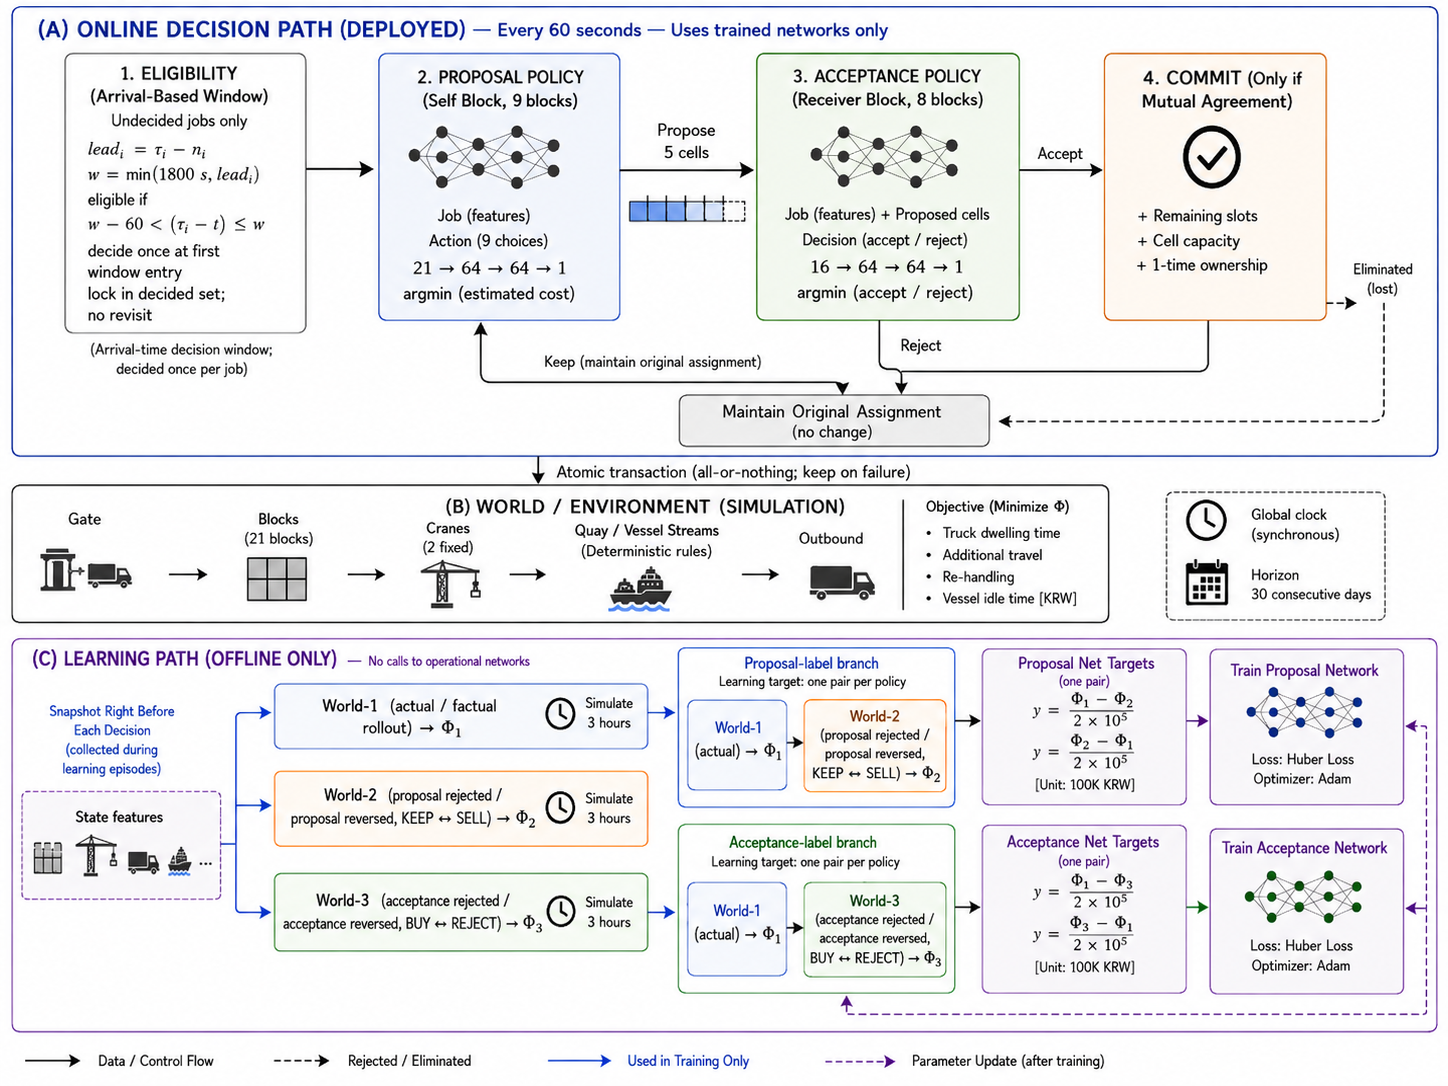
\includegraphics[width=\textwidth]{system-architecture.png}
\caption{(a) Every 60\,s, the online path checks eligibility,
proposal, acceptance, and commitment. (b) The simulator links gate,
blocks, cranes, and vessels to cost $\Phi$. (c) Offline learning compares
up to three worlds from the same state and random stream over 3\,h
to label the two networks.}
\label{fig:arch}
\end{figure}
\subsection{Notation, Actions, and Policies}
\label{sec:arch-notation}
Every $\delta=60$\,s, eligible announced jobs are reviewed once.
Job $i$ has assignment $z_i=(b_i,\tau_i)$ and legal actions
$a_i=(b'_i,\Delta_i)\in\mathcal A_i(t)$, producing
$z_i(a_i)=(b'_i,\tau_i+\Delta_i)$. KEEP is $a_i^0=(b_i,0)$.
Full selects among spatial and temporal alternatives; each changed
candidate alters one axis: block or arrival delay ($\Delta_i>0$).
Outbound jobs retain their assigned block. Let $n_i$ be announcement
time, $g_i$ gate-in time, and $r_i$ the prior-review indicator. With
$W=1800$\,s and $w_i=\min(W,\tau_i-n_i)$, eligibility is
\begin{equation}
\mathcal E_t=\{i\mid w_i-\delta<\tau_i-t\le w_i,\ \tau_i>t,\ g_i>t,\ r_i=0\}.
\end{equation}
Review occurs within one decision interval after entering this window,
approximately $W$ before arrival when notice is sufficiently early.
Jobs announced at or after arrival are ineligible; the lead-time model
assigns 14.1\% of demand to that category. This review window is an
algorithmic choice, not a validated carrier notification allowance.
The proposal policy scores
each candidate from the block state and job-action features $o_i^P$ and
selects the lowest score, while the acceptance policy compares
acceptance with rejection from the proposal message and the destination
state $o_i^A$:

\begin{equation}
\begin{aligned}
\hat a_i&=\arg\min_{a\in\mathcal A_i(t)}
\hat c_{\theta}^{P}(o_i^P,a),\qquad
p_i=\mathbf 1[\hat a_i\ne a_i^0],\\
q_i&=\mathbf 1\!\left[
\hat c_{\psi}^{A}(o_i^A,\hat a_i,\mathrm{acc})
\le
\hat c_{\psi}^{A}(o_i^A,\hat a_i,\mathrm{rej})
\right].
\end{aligned}
\end{equation}
If the target resource has no remaining capacity, the request is
rejected before the network is called. The mutually accepted candidates
form $\mathcal J_t=\{i\in\mathcal E_t\mid p_iq_i=1\}$.

\subsection{Central Commitment}
\label{sec:arch-commit}
The central procedure creates no new candidates. It considers only
$\mathcal J_t$, ordered by the acceptance policy's predicted score with
lexicographic tie-breaking. The pair-centred scores are not calibrated
across jobs (Sect.~\ref{sec:arch-labels}). Their order is deterministic,
but can change which proposals obtain a contested resource; it is
therefore an algorithmic priority, not a validated ordering of monetary
benefits. Its effect must be separated from the acceptance veto. With $x_i\in\{0,1\}$ indicating commitment,
$F_b(t)$ the free slots in block $b$, and $K_k(t)$ the remaining quota
of time slot $k$, it enforces

\begin{equation}
\begin{aligned}
x_i&\le p_iq_i,\qquad
\sum_{i\in\mathcal J_t}\!x_i\mathbf1[b'_i\!=\!b]\le F_b(t),\\
\sum_{i\in\mathcal J_t}\!x_i\mathbf1[k(i)\!=\!k]&\le K_k(t),\qquad
\sum_{t\in\mathcal T}\!\mathbf1[i\in\mathcal E_t]\le1.
\end{aligned}
\end{equation}
Block-capacity checks are applied, but $K_k(t)=\infty$ in all reported
experiments because terminal-specific booking quotas are unavailable.
The candidate time range is an algorithmic setting, not a verified
carrier availability window or notification allowance. Thus these
checks establish feasibility only within the simulated rules, not
the executability of a changed appointment in practice. All committed assignments are applied together at the end of
the decision epoch, so an earlier commitment cannot change the state
seen by another candidate in the same epoch.

\subsection{Cost Networks}
\label{sec:arch-models}
Both $\hat c^{P}_{\theta}$ and $\hat c^{A}_{\psi}$ are multilayer
perceptrons with two 64-unit hidden layers and ReLU, with weights shared
across blocks: $21\to64\to64\to1$ for proposal and $16\to64\to64\to1$
for acceptance, or fewer than 11{,}000 parameters in total. Inputs
include current waiting, inventory, remaining crane work, the public
expected arrival time, route difference, and announced volume near the
target time; unrealised arrival and completion times and simultaneous
responses from other accepting parties are excluded. The output is one
pair-centred cost score per candidate, so the length of the candidate
list may change without retraining. Pair centring preserves the ordering
inside one pair, but does not by itself justify all comparisons in~(2).
For a fixed state and a common KEEP outcome $K=C(s,\mathrm{KEEP})$,
the ideal label of a changed candidate is
\begin{equation}
y(s,a)=\frac{C(s,a)-K}{2S},\qquad S=100{,}000\;\mathrm{KRW}.
\end{equation}
Changed candidates preserve their true cost order only when the state,
exogenous trajectory, continuation policy, and horizon share that same
reference. The learned predictions need not preserve it. Moreover,
KEEP's target $(K-C(s,a))/(2S)$ depends on the paired alternative,
even when its input is unchanged. Ordering changed candidates and
deciding against a learned KEEP score are therefore distinct validation
questions. This conditional explanation does not establish measured
ranking accuracy.

\subsection{Counterfactual Cost Labels and Training}
\label{sec:arch-labels}
For each sampled decision we clone the state and the random stream just
before branching and run up to three worlds for $H=10{,}800$\,s:
$\phi_i^F=\Phi_H(\text{observed})$,
$\phi_i^P=\Phi_H(\text{proposal reversed})$, and
$\phi_i^A=\Phi_H(\text{acceptance reversed})$. The counterfactual branch
reverses the policy's observed decision: if the proposal policy proposed
a change the alternative keeps the assignment; if it kept the assignment,
the alternative forces a proposal selected by the current weights.
Acceptance and feasibility still govern actual commitment. The acceptance
alternative swaps acceptance and rejection.
For each policy the two actions of the pair are centred on their mean
and divided by KRW 100{,}000,

\begin{equation}
\bar\phi_i^P=\frac{\phi_i^F+\phi_i^P}{2},\quad
y_{i,F}^P=\frac{\phi_i^F-\bar\phi_i^P}{10^5},\quad
y_{i,P}^P=\frac{\phi_i^P-\bar\phi_i^P}{10^5},
\end{equation}
that is, $\pm$ half the pairwise cost difference; the same centring is
applied to $(\phi_i^F,\phi_i^A)$. The reference point is therefore the
pair itself rather than a fixed action.
We sample at most 64 decisions per day, split them 80/20 into training
and validation, and optimise with Adam ($3\times10^{-4}$) and Huber loss
($\beta=1.0$), which prevents a few very large counterfactual
differences from dominating the fit~\cite{refhuber}. Exploration
decreases linearly from 0.50 to 0.05 over the 30 training iterations.
States and alternatives change with the current policy; each iteration
discards its labels after updating. This is finite-horizon Monte-Carlo
cost learning with simulator-generated baselines, without target
bootstrapping or a policy-gradient update.
Training both networks for 30 iterations took about 18 hours
of wall-clock time. During evaluation the weights are frozen,
exploration is disabled, and no counterfactual branch is called, so
network scoring is only part of the online path. Candidate construction,
conflict resolution, and commitment must also be timed.

\subsection{Intended Users and Operational Context}
\label{sec:user-context}
Terminal yard planners and operations staff are the intended users,
with carrier dispatchers and drivers. Busan New Port waiting-time
research~\cite{refbusanwait}, Korean terminal operating system (TOS)
research~\cite{reftos}, and the Busan Port Authority's AllCON-e booking
and information services~\cite{refallcone} motivate this proposed
application; integration is untested.

A planner would compare the original and recommended block/time and
observed congestion, then accept, modify, or reject the recommendation.
A carrier dispatcher would check vehicle availability and subsequent
jobs, negotiate an acceptable window, or decline. The driver would
receive the agreed assignment and report execution difficulties.
Operator review precedes carrier agreement and driver notification;
without agreement, the original assignment remains pending review.
Human response deadlines are separate from the 60-second review interval.

Network acceptance is not human consent, and scores are not calibrated
monetary savings or confidence probabilities. The evaluated decision
engine supplies no evidence about interfaces, usability, or human
acceptance; these require integration and user evaluation.

\section{Experimental Environment and Evaluation Protocol}
\label{sec:env}
The synthetic setting draws on reported block counts~\cite{ref16},
cranes~\cite{ref8}, multi-week operation and handling times~\cite{ref9},
and arrival variation~\cite{ref13}. Table~\ref{tab:setup} distinguishes
design choices from literature-informed values~\cite{ref20}; it does
not reproduce a particular terminal. The generator's 45\% initial fill
corrects the earlier 65\% manuscript entry, not a new occupancy experiment.
\begin{table}[bp]
\centering
\caption{Simulation and learning settings. Design values, including
literature-informed conversions, are not measurements at a specific
terminal. Historical and revision evaluations are listed separately.
Requested arrival times follow
$f(t)=0.38\,U(0,24)+0.62\sum_{m=1}^{3}w_m\mathcal N(t;\mu_m,\sigma_m^2)$
with $(\mu_m,\sigma_m,w_m)$ equal to $(10,1.5,.317)$, $(15,2.5,.633)$,
and $(21,1,.05)$, time in hours.}
\label{tab:setup}
\small
\setlength{\tabcolsep}{4pt}
\begin{tabular}{@{}l l@{\hspace{0.9em}} l@{}}
\toprule
Group & Setting & Value \\
\midrule
Yard & Blocks, cranes per block & 21, 2 \\
 & Slots per block, initial fill (design) & 1{,}440, 45\% \\
\midrule
Time & Decision interval $\delta$ & 60\,s \\
 & Review window $W$ & 1{,}800\,s \\
 & Counterfactual horizon $H$ (design) & 10{,}800\,s \\
\midrule
Demand & Announcement lead & median 1.27\,h (14.1\% $\le0$) \\
 & Daily levels (design) & 3{,}500, 5{,}000, 7{,}500, 12{,}500, 15{,}000 \\
 & Draw probabilities (design) & 0.30, 0.30, 0.25, 0.10, 0.05 \\
 & Arrival curve (design) & uniform base 38\% $+$ 3 Gaussians \\
\midrule
Vessels & Classes (GT), calls/day, crane rate & 50/100/150k, 3.3, 27.5 moves/h \\
\midrule
Cost & Truck dwell (design) & KRW 40{,}000/h (twice beyond 1\,h) \\
 & Crane move, rehandle (design) & KRW 60{,}000/h, KRW 2{,}000/event \\
 & Vessel idling & KRW 2.99 per GT-hour~\cite{ref25} \\
\midrule
Learning & Networks (proposal, acceptance) & $21/16\!\to\!64\!\to\!64\!\to\!1$ \\
 & Iterations, decisions per day & 30, $\le64$ \\
 & $\varepsilon$, optimiser & $0.50\!\to\!0.05$, Adam $3\times10^{-4}$ \\
\midrule
Evaluation & Historical days, compared, seed & 30, middle 28, 9{,}900{,}950 \\
 & Registered revision & 20 months, 4 fixed-policy variants \\
 & Policy at evaluation & frozen weights, $\varepsilon=0$ \\
\bottomrule
\end{tabular}
\end{table}
The cost attributed to day $d$ has four terms. Truck costs follow
the original requested day, while the other terms follow calendar
time; consequently this is not a purely calendar-day cash-flow total.
Here $h_i$ is
the dwell time of truck $i$, $m$ the additional crane working time, $R$
the number of rehandles, and $T_v$ the policy-related idle time of
vessel $v$:

\begin{equation}
\begin{aligned}
\Phi_d&=C_{wait,d}+C_{move,d}+C_{rehandle,d}+C_{vessel,d},\\
C_{wait}&=\sum_i 40{,}000\{h_i+\max(0,h_i-1)\},\qquad
C_{move}=60{,}000\,m,\\
C_{rehandle}&=2{,}000\,R,\qquad
C_{vessel}=\sum_v 2.99\,GT_v T_v.
\end{aligned}
\end{equation}
The base monetary scale is
derived from the safe trucking freight rate~\cite{ref24}, whereas the
conversion to an hourly dwell-cost coefficient is a design choice.
Structural vessel time that the policy cannot change is recorded
separately. Truck dwell is measured after gate entry; the objective
does not include waiting outside the gate, carrier rescheduling
charges, or disruption to subsequent trips. These omitted burdens
can change the net benefit of a time adjustment. In the historical run,
truck waiting contributes 96.4\% of cost, making results especially
sensitive to its coefficient and the excluded external burdens.

\subsection{Historical Run and Independent Evaluation}
\label{sec:independent-protocol}
Historical results use one continuous 30-day trajectory (seed
9{,}900{,}950), measured over days 2--29. Common exogenous streams
support matched comparisons~\cite{ref22}, but state carries across
days. Daily wins are descriptive; day-level tests and day-resampled
intervals are not independent-replication evidence. The first-iteration
checkpoint already contains one update and is not an untrained model.

The revision fixes 20 seeds, starting at 20{,}000{,}000 with spacing
100{,}000. Each policy--seed run starts a fresh engine for 30 continuous
days plus the existing two-hour closing interval. Arrival curves,
daily-volume probabilities, truck attributes, and initial inventory
are preserved and matched within seeds. Weights are fixed; exploration,
updates, and training branches are disabled. This evaluates variation
across environments for one model, not across training runs.

Legacy admission could omit requests lacking stock or reservations.
The revision registers all requests and shares a fixed correction to
selected vessel loading/discharging directions across policies,
recording both input versions.
Historical and revised costs are not pooled. Completed, unfinished,
and unbound requests and vessel work accompany costs; valid records
do not imply full service. Outbound jobs retain their block, but
synthetic targets may be rebound within it rather than representing
fixed customer-container identities.

No reallocation, Full, and Time-only comprise the original 60 runs.
Block-only adds the same 20 seeds, totalling 80 runs, under a separate
17 September registration after one baseline month and partial results
were available. All variants share the checkpoint; action restrictions
are not separately optimised policies. The comparison families remain
separate.

For policy $p$ and seed $s$, let $C_{p,s}$ be the cost over the
28 measurement days. The two original primary differences are
\begin{equation}
D_s^{B}=C_{\mathrm{baseline},s}-C_{\mathrm{Full},s},\qquad
D_s^{T}=C_{\mathrm{Time},s}-C_{\mathrm{Full},s}.
\end{equation}
Positive values favour Full. We resample the 20 paired months
20{,}000 times (seed 9{,}900{,}721), retaining within-month dependence.
Each primary mean difference has a 97.5\% percentile interval;
secondary intervals are descriptive 95\%. The separate Block-only
family uses seed 9{,}900{,}723 and 97.5\% intervals for baseline minus
Block-only and Block-only minus Full. Two separate families do not
provide one four-claim error guarantee. Supplementary 30-day totals
are not longer simulations. Per-seed costs, percentage savings,
aggregate ratios, wins/ties/losses, and residuals require complete
matched sets with no outcome-based sample changes. Results are pending.

Daily records contain volume, starting backlog, block queues, unfinished
crane work, mean/90th-percentile truck turn time, action counts, and
costs. Planned demand defines descriptive groups; realised queues
interpret congestion without redefining groups after observing outcomes.
The 600 days are not independent replications.

\section{Results and Evidence Status}
\label{sec:exp}
\subsection{Historical Cost Comparison}
\label{sec:exp-paired}
Table~\ref{tab:main} preserves the legacy single-run results:
approximately KRW 10.00\,billion without reallocation and
KRW 8.52\,billion with Full over 28 days. They use the historical
contract, not the ongoing independent evaluation.
\begin{table}[htbp]
\centering
\caption{Historical 28-day comparison. Positive reduction means lower
recorded cost than no reallocation. Daily wins are descriptive, without
independent-sample significance; dashes denote unreported values.}
\label{tab:main}
\small
\setlength{\tabcolsep}{5pt}
\begin{tabular}{@{}llrc@{}}
\toprule
Policy & Actions & Reduction & \shortstack{Full cheaper\\(days)} \\
\midrule
\textbf{Full} & block+time & \textbf{+14.72\%} & --- \\
Time-only & time & +13.44\% & --- \\
Block-only & block & $-$1.31\% & --- \\
First-iteration model & block+time & +7.97\% & 18/28 \\
\midrule
Rule: least-loaded slot & time & +3.41\% & --- \\
Rule: least-loaded block+slot & block+time & +1.51\% & 20/28 \\
Rule: least slack & block & +0.53\% & 20/28 \\
Rule: first-come-first-served & block & +0.17\% & 22/28 \\
Rule: shortest processing time & block & +0.05\% & 21/28 \\
Rule: net gain & block & $-$0.48\% & 21/28 \\
\midrule
No reallocation & --- & 0.00\% & 26/28 \\
\bottomrule
\end{tabular}
\end{table}

Full's additional reduction over Time-only is only 1.28 percentage
points relative to the baseline. Block-only increases aggregate cost.
Neither finding establishes a general need for spatial adjustment;
the registered direct month-level comparison addresses that question.
The least-loaded-slot rule saves 3.41\% without learning. Historical
Time-only is cheaper than this rule on just 8/28 days, yet has a lower
aggregate cost by about KRW 1.00\,billion. This illustrates why frequency
of wins and magnitude of savings must be reported together, without
treating dependent days as independent evidence.

\subsection{Demand Level and Action Contributions}
\label{sec:exp-decomp}
\begin{figure}[htbp]
\centering

\includegraphics[width=\textwidth]{fig-decomposition.pdf}
\caption{Historical cost reduction by planned demand, in million KRW.
Bars compare each restricted policy with no reallocation; the diamond
compares Full with the first-iteration checkpoint. The shaded demand
levels contain four days. Groups have unequal numbers of dependent
days; their totals are descriptive, not comparable daily averages.}
\label{fig:decomp}
\end{figure}
Four high-volume days contribute 90.5\% of historical savings.
Time-only and Block-only save 1.344 and $-0.131$ billion KRW,
respectively. The interaction residual of 0.258 billion KRW is
arithmetic, not a verified component effect. Block-only saves cost at
3{,}500 and 5{,}000 trucks but loses at 15{,}000, where Time-only beats
Full by approximately KRW 25\,million. Spatial benefits are therefore
conditional. Volume alone does not establish congestion when backlog
persists across days.

The existing sweep varies high-volume days at 2, 6, and 14 out of 28
on seed 9{,}900{,}980. Time-only accounts for 67\%, 79\%, and 81\%
of Full's savings. Spatial action shares, recalculated over the same
28 days, are 31.60\%, 20.77\%, and 11.16\%. The four-day case uses a
different seed and is not a fourth controlled point. This sweep does
not validate other peak widths, costs, or horizons, or a hand-written
low/high-congestion switching rule.

\subsection{Learning Diagnostics}
\label{sec:exp-learning}
\begin{figure}[htbp]
\centering

\includegraphics[width=\textwidth]{fig-learning-curve-2p.pdf}
\caption{Historical training and validation losses over 30 iterations.
Thin lines are iteration values and thick lines five-iteration means;
the vertical axis is logarithmic. Shading marks demand at least
12{,}500. These diagnostics concern one training trajectory, not
independent training replications or full-candidate ranking accuracy.}
\label{fig:learn}
\end{figure}
From the first to last five iterations, proposal training and validation
losses fall from (0.079, 0.268) to (0.029, 0.119); acceptance losses
fall from (0.171, 0.315) to (0.027, 0.136), using 4{,}671
counterfactual worlds. Pair-fit diagnostics do not prove global ranking.
The first-iteration checkpoint costs KRW 9.20\,billion; later updates
save another KRW 0.675\,billion, 94.6\% on four high-volume days.
This requires independent runs, not post-hoc selection of favourable
days. Day-resampled intervals do not establish learning effects, and
frozen-model evaluation does not test training-seed stability.

\subsection{Outstanding Evidence and Reporting Boundaries}
\label{sec:pending-evidence}
The 80-run comparison remains in progress; no independent estimate or
interval is supplied here. Costs require joint interpretation with
completed and unfinished work. The four policies do not isolate the
acceptance network: veto removal retains score-based ordering.
A separate ablation must distinguish these functions while preserving
physical feasibility checks.

Candidate ranking remains unvalidated. Tests must compare KEEP and all
legal actions from the same held-out state, external inputs, continuation
policy, and horizon. Outcomes include selection regret (selected cost
minus the minimum candidate cost), best-action selection, and ranking
agreement. Exact action execution and factual replay across day
boundaries must first be verified.

Online latency is unmeasured. State and candidate construction, features,
scoring, conflict resolution, and commitment need timing apart from
simulation advancement, with hardware, threads, candidate counts,
warm-up, median, upper percentiles, maximum, and 60-second overruns.
Network size and month runtime are not latency evidence.

The one-axis synthetic layout does not validate distinct horizontal
and vertical handling systems. Their travel paths, transfer points,
and crane-resource sharing require explicit comparison; rotating
coordinates is insufficient. Hybrid layouts are excluded. Cost-weight,
peak-width, and longer-run robustness also remain untested by the
existing frequency sweep.

\section{Conclusion}
\label{sec:concl}
Separate proposal and acceptance policies learn from counterfactual
cost differences to revise spatial--temporal assignments. Historical
savings are concentrated in high-volume days, with conditional spatial
contributions. Consistent improvement, component necessity, and
operational feasibility remain unestablished; the independent-month
results are pending.

Deployment would require finite booking quotas, carrier-approved
windows, minimum notification time, and cargo/vessel deadlines in a
feasibility layer~\cite{ref4,ref6,refquota}, together with external
waiting, rescheduling, and subsequent-trip costs. Those require
terminal and carrier data. We have not tested savings under those
constraints or estimated a break-even rescheduling charge. Remaining
work includes candidate ranking, acceptance ablations, cost and horizon
sensitivity, online timing, and distinct basic layouts. TOS and
AllCON-e provide an application context; the proposed operator--carrier--
driver workflow still requires integration and user evaluation.

\begin{credits}
\subsubsection{\ackname}
This work was supported by the Public-Private Joint Technology
Commercialization R\&D program (Technology Transfer and
Commercialization, RS-2026-25529952) funded by the Ministry of SMEs and
Startups (MSS, Korea).

\subsubsection{\discintname}
The authors have no competing interests to declare that are relevant to
the content of this article.
\end{credits}

% =====================================================================
\small
\begin{thebibliography}{22}
\raggedright
\setlength{\itemsep}{0pt}
\setlength{\parsep}{0pt}
\setlength{\topsep}{2pt}
\bibitem{ref1} Yen, B.T.H., Huang, M.J., Lai, H.J., Cho, H.H., Huang, Y.L.: How smart port design influences port efficiency: a DEA-Tobit approach. Res. Transp. Bus. Manag. \textbf{46}, 100862 (2023)
\bibitem{ref4} Chen, G., Govindan, K., Yang, Z.: Managing truck arrivals with time windows to alleviate gate congestion at container terminals. Int. J. Prod. Econ. \textbf{141}(1), 179--188 (2013)
\bibitem{ref6} Phan, M.-H., Kim, K.H.: Collaborative truck scheduling and appointments for trucking companies and container terminals. Transp. Res. B \textbf{86}, 37--50 (2016)
\bibitem{ref7} Ng, W.C., Mak, K.L.: Yard crane scheduling in port container terminals. Appl. Math. Model. \textbf{29}(3), 263--276 (2005)
\bibitem{ref8} Speer, U., Fischer, K.: Scheduling of different automated yard crane systems at container terminals. Transp. Sci. \textbf{51}(1), 305--324 (2017)
\bibitem{ref9} Petering, M.E.H., Murty, K.G.: Effect of block length and yard crane deployment systems on overall performance at a seaport container transshipment terminal. Comput. Oper. Res. \textbf{36}(5), 1711--1725 (2009)
\bibitem{ref16} Schwientek, A., Lange, A.-K., Jahn, C.: Simulation-based analysis of dispatching methods on seaport container terminals. In: ASIM Symp. Simulationstechnik (SST 2020). ARGESIM Report, vol.~59, pp. 357--364 (2020)
\bibitem{ref19} Wang, W., Liu, H., Peng, Y., Cao, Z., Yu, P., Lu, Z.: Yard crane real-time scheduling among multi-block at terminal: A reinforcement learning based proximal policy optimization approach. Transp. Res. E \textbf{207}, 104635 (2026)
\bibitem{ref10} Wolpert, D.H., Tumer, K.: Optimal payoff functions for members of collectives. Adv. Complex Syst. \textbf{4}(2--3), 265--279 (2001)
\bibitem{ref11} Foerster, J.N., Farquhar, G., Afouras, T., Nardelli, N., Whiteson, S.: Counterfactual multi-agent policy gradients. In: Proc. 32nd AAAI Conf. Artif. Intell. pp. 2974--2982. AAAI Press (2018)
\bibitem{ref13} Kourounioti, I., Polydoropoulou, A.: Application of aggregate container terminal data for the development of time-of-day models predicting truck arrivals. Eur. J. Transp. Infrastruct. Res. \textbf{18}(1), 76--90 (2018)
\bibitem{refquota} Huynh, N., Walton, C.M.: Robust scheduling of truck arrivals at marine container terminals. J. Transp. Eng. \textbf{134}(8), 347--353 (2008). doi:10.1061/(ASCE)0733-947X(2008)134:8(347)
\bibitem{refmnih} Mnih, V., et al.: Human-level control through deep reinforcement learning. Nature \textbf{518}(7540), 529--533 (2015)
\bibitem{refhornik} Hornik, K.: Approximation capabilities of multilayer feedforward networks. Neural Netw. \textbf{4}(2), 251--257 (1991)
\bibitem{refhuber} Huber, P.J.: Robust estimation of a location parameter. Ann. Math. Statist. \textbf{35}(1), 73--101 (1964)
\bibitem{refbusanwait} Kim, Y.-I., Shin, J.-Y., Park, H.-J.: A study on the prediction of gate in-out truck waiting time in the container terminal. J. Navig. Port Res. \textbf{46}(4), 344--350 (2022). doi:10.5394/KINPR.2022.46.4.344 (in Korean)
\bibitem{reftos} Won, S.-H., Cho, S.-W., Lee, E.-K.: Analysis technology trend and strategies to vitalize the industry on terminal operating system (TOS) of smart port. J. Shipping Logist. \textbf{41}(1), 25--53 (2025). doi:10.37059/tjosal.2025.41.1.25 (in Korean)
\bibitem{refallcone} Busan Port Authority: Handle Busan Port container cargo easily with AllCON-e. Press release, 16 August 2022 (in Korean; title translated). \url{https://www.busanpa.com/board/view.do?boardId=BBS_0000031&dataSid=27966&menuCd=DOM_000000105002001000}
\bibitem{ref20} Kim, S., Mowakeaa, R., Kim, S.-J., Lim, H.: Building energy management for demand response using kernel lifelong learning. IEEE Access \textbf{8}, 82131--82141 (2020)
\bibitem{ref25} Ministry of Oceans and Fisheries: Regulations on the Use of Port Facilities and Fees at Trade Ports, etc. MOF Notice No. 2025-218 (2025) (in Korean)
\bibitem{ref24} Ministry of Land, Infrastructure and Transport: Notice on Safe Freight Rates for Cargo Vehicles Applicable in 2026. MOLIT Notice No. 2026-402 (2026) (in Korean)
\bibitem{ref22} Kleijnen, J.P.C.: Analyzing simulation experiments with common random numbers. Manag. Sci. \textbf{34}(1), 65--74 (1988)
\end{thebibliography}

\end{document}
